\section{Introduction} \label{sec:intro}

% lineeaari tv -> videonauhuri -> on demand -> on demand tv
Before videocassette recorders became widely available for regular households, watching television was a very time-sensitive activity, if you wanted to see a TV program you had to watch it when it was broadcasted. When video recorders became affordable, they enabled people to record and watch TV programs whenever they wanted. Currently, linear TV is losing even more of its foothold, as various video-on-demand services are gaining popularity. % at the expense of broadcast TV.
Recording storage is also moving away from the homes of viewers into the cloud servers of content providers.

% NVPR = videonauhuri pilvessä, jonka katsoja jakaa muiden kanssa
Network personal video recorder (NPVR) is a type of service for recording broadcast TV programs for later viewing. Instead of storing recordings on the users local device, NPVR stores recordings on the content providers server. For every program listed in the Electronic program guide (EPG), a single recording is created and stored on the server. The users who record the same program will receive the same video from the server.

% NPVR ongelma
The NPVR recording start and end times are determined by the scheduling information given in the EPG. However, it is common that programs are not broadcasted exactly according to the EPG schedule. To ensure that the whole program is recorded, some margin is typically added on both ends of the recording. Thus, NPVR recordings tend to have some non-program content at the beginning and end, in which the users are not interested in. %This extra content is generally uninteresting to the users.
Furthermore, some programs have also advertisement breaks, which the users typically also want to avoid watching.
%The goal of this thesis is to study whether user viewing behaviour can be used to determine where the start and end credits begin in an NPVR recording.

% motivaatio
I am writing this thesis for a  NPVR service provider company. From the perspective of an NPVR service provider, detecting advertisement breaks and start and end credits is useful for the following reasons. Firstly, less storage space is needed if the surplus contet is discarded. Secondly, it is convenient for the customers if they do not have to search for the relevant content in a recording.
%Secondly, when the customers want to watch multiple episodes of a series in a row, it is convenient for them if a link to the next episode is displayed during the closing credits.

% rajaus
% User viewing behaviour might also be useful for detecting starting credits and advertisement breaks, but on this thesis I will focus on the closing credits detection to narrow down the topic. I will also restrict the examined recordings to TV series with multiple episodes and at least one hundred views per episode.

% sisältö ja rakenne
The main goal of this thesis is to study whether user viewing behaviour can be used to detect start and end credits and advertisement breaks of NPVR recordings.
The thesis is structured as follows. Section 2 gives an overview of the characteristics of the viewing behavioiur data. Section 3.1 discusses the theoretical background of signal change point detection from the viewpoint of this specific use case. Result evaluation and validation is discussed in section 3.2. In section 4.1 the Python scientific library \texttt{ruptures} is used to detect closing credits. The results are evaluated in section 4.2. Section 5 discussion considers, based on the previous sections, the viability of using user viewing behaviour for closing credits detection. Lastly, the main points of this thesis are summarised in section 6 conclusions.

\section{User viewing behaviour data} \label{sec:data} % or use case, signal type, data properties etc.

\subsection{Structure of the data} \label{subsec:data}
The content of an NPVR video recording can be categorised into core program content, start credits, advertisement breaks, end credits and non-program content at the very beginning and end of a recording. Core program content is considered relevant for the users, while non-program content and advertisement breaks are considered irrelevant. The relevancy of start and end credits is something in between, since many users prefer to skip them, but they still belong to the program and are not extra content as such.

For the purpose of this thesis, starting credits, advertisement breaks and end credits will be referred to as change points. The goal of this thesis is to find a method to determine at least the approximate location of change points, and preferably even the start and end timestamps of change points with some small margin of error.

\begin{figure}[H]
    \centering
    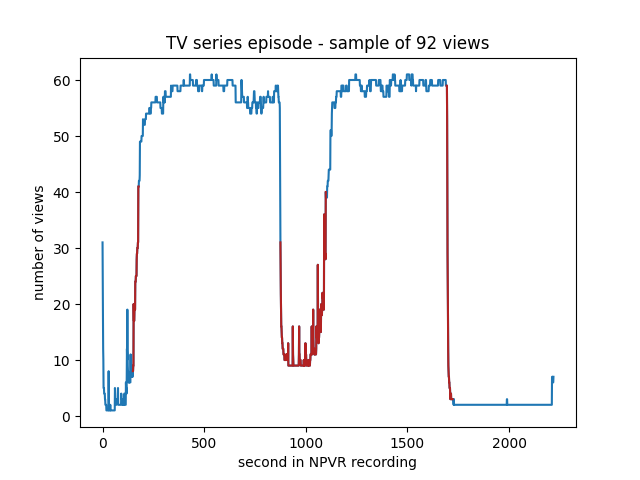
\includegraphics[width=1\textwidth]{../plots/episode.png}
    \caption{Visualisation of user views count for each second in an example NVPR recording}
    \label{fig:intro_ads_outro}
    \end{figure}

An example of user viewing behaviour data is illustrated in Figure \ref{fig:intro_ads_outro}.The sample consists of 92 user views of an NPVR recording. The horisontal axis contains one second-long intervals, corresponding to each second of the recording. The vertical axis shows how many times a second-long interval in the recording was viewed by users. For example, 58 users from the sample of 92 users watched the part of the video between 0:10:00 - 0:10:01 (600 on the horisontal axis in Figure \ref{fig:intro_ads_outro}).

The change points are marked on the plot in red. In Figure \ref{fig:intro_ads_outro} there are a total of three change points, which correspond to start credits, advertisement break and end credits, respectively. The beginning and end timestamps of the change points were checked by hand from the video recording. It can be seen from the plot that a steep increase in views occurs when the actual program content begins, and correspondingly there is a steep decrease in views when the program content shifts to advertisements or closing credits.

%The starting credits, advertisement break and closing credits are marked on the plot in red. Their beginning and end times were checked by hand from the video recording. A steep increase in views occurs in the plot whenever the actual program content begins, and correspondingly there is a steep decrease in views when the program content shifts into to advertisements or closing credits.

\subsection{Ground truth} \label{subsec:groundtruth}

In order to evaluate how well a method detects change points, a ground truth is needed for comparison. The ground truth is obtained by having a person look at the video recording and having them write down the timestamps of the change points.

I have collected the start and end times of the change points from 155 NPVR recordings by hand with a margin of error of $\pm$ 1 seconds. Each of these recordings has at least one hundred user views.

\section{Theoretical background} \label{sec:background}

\subsection{Signal change detection} \label{subsec:methods} % for this specific case

%definition
%classification:
%methods (the paper, bayes, something else)
%online/offline
%(un)known nof points 
%cost function, parametric/non-parametric
%search method, optimal/approximate (accuracy vs performance)

%tie to npvr case & definition
Locating the content change points from user behaviour data can be formulated as a signal processing problem, more precisely as a change point detection problem. Signal change point detection is quite widely researched topic, since it has applications in multiple fileds such as ... % TODO: add examples

% offline
Change point detection problems can be divided into two main categories, depending on whether the change detection must be done for incoming data in near real-time, or not. Methods solving the former case are referred to as online algorithms. Offline algorithms solve the latter case, and they differ from the online algorithms by getting the entire dataset as input and typically being more computationally complex, but also by detecting the changes more accurately.

% unknown number of changes
Offline methods can be divided into two categories, based on whether the number of changes in the dataset is known beforehand, or not. If the number of change points is not known, an extra step is needed to determine it. There are multiple methods for doing this.


\subsection{Result evaluation and validation} \label{subsec:validation}

% specific to change point detection:

% Annotation error
% kuinka paljon mallin antamien muutospisteiden määrä eroaa todellisesta määrästä

% Hausdorff
% kuinka suuri on isoin ero mallin antamasta muutoskohdasta lähimpään todelliseen muutoskohtaan

% Rand index
% kuinka suuren osan koko otoksesta malli on luokitellut oikein

% F1-Score
% precision (kuinka suuri osa löydetyistä todellisia), recall (kuinka suuri osa todellisista löydetty)

% general:

\section{Empirical research} \label{sec:casestudy}

\subsection{Change point detection with \texttt{ruptures} library} \label{subsec:solution}
% cost-function -> probably non-parametric (distribution not known)
% search method -> probably optimal (pelt) but approximate methods could be tried
% constraint -> unknown K^* 

A Python library called \texttt{ruptures} will be used for the change point detection. \texttt{ruptures} is based on the findings of a literature reviw conducted by Truong et al. \cite{truongSelectiveReviewOffline2020} which examines various methods for offline change point detection. Selected algorithms examined in the literature review are implemented in \texttt{ruptures}.

Choosing the most suitable algorithm %from the library
for this use-case can be done by considering the three aspects of change detection methods discussed in the literature review: cost-function, search method and constraint. Accuracy is more important than low computational complexity, so optimal method is preferable to an approximate one. As the number of change points is unknown, the only suitable optimal search method is \texttt{Pelt}. The algorithm was first indroduced by Killick et al. \cite{killickOptimalDetectionChangepoints2012}.

An example of \texttt{Pelt} output is visualised in Figure \ref{fig:ruptures_change_detection}. The input data is the same as in Figure \ref{fig:intro_ads_outro}. Red rectangles on the plot represent the actual location of the starting credits, advertisement break and closing credits, respectively. The vertical dashed lines indicate the change points determined by Rupture. They appear to be very close to the genuine change points at the edges of the red blocks.

\begin{figure}[H]
\centering
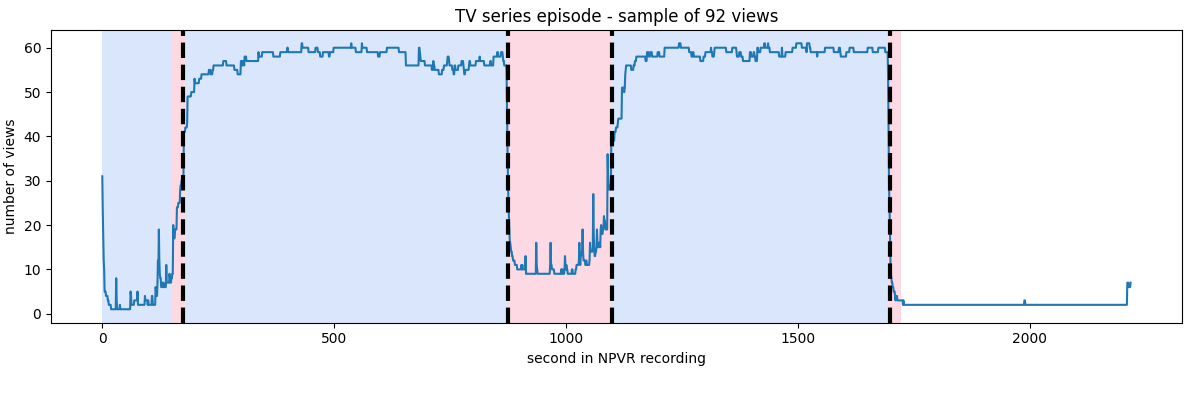
\includegraphics[width=1\textwidth]{../plots/episode-pen100.png}
\caption{\texttt{Pelt} output for Figure \ref{fig:intro_ads_outro} data}
\label{fig:ruptures_change_detection}
\end{figure}

\subsection{Results} \label{sec:results}

\section{Discussion} \label{sec:discussion}

\section{Conclusions} \label{sec:conclusions}
